\documentclass{beamer}
\mode<presentation>
{
  \usetheme[height=40pt]{ScarletHannover} %UNL-Sbaush, MyHannover, BlueHannover, ScarletHannover, Lart
  \useinnertheme[shadow=true]{rounded}
  %\useoutertheme{shadow}  
   \usefonttheme{professionalfonts}
  %\usefonttheme{structureitalicserif,structuresmallcapsserif,professionalfonts,serif,structurebold,}
   
   %\usecolortheme{sbaushOUTER} % ---> OUTER
   %\usecolortheme{sbaushINNER} % ---> INNER
   %\usecolortheme{fly}    % ---> COMPLETE
 
%\usecolortheme{default,structure,sidebartab,albatross,dove,fly,seagull,crane,beetle}

%\INNER --> usecolortheme{lily,orchid,rose,}
%\OUTER --> usecolortheme{whale,seahorse,dolphin,}

\setbeamertemplate{navigation symbols}{}
  \setbeamercovered{transparent}
}
\usepackage[italian]{babel}
\usepackage[utf8]{inputenc}
\usepackage{times}
\usepackage{listings}
\usepackage[T1]{fontenc}
\usepackage{graphicx}
\usepackage{epsfig}
%\usepackage{beamerouterthemeleo}
%\usepackage{algorithmic}
%\usepackage{algorithm}
%%%%%%%%%%%%%%%
% Definitions %
%%%%%%%%%%%%%%%



%\newcommand{\g}[1]{\alert{#1}}

\institute[Università degli studi di Firenze, Facoltà di Ingegneria] % (optional, but mostly needed)
{
\begin{minipage}[t]{0.4\textwidth}
 \textbf{Docente:} \\ \professor \\
\textbf{Assistenti:} \\ \firstassistant \\  \secondassistant
\end{minipage} 
\hfill
\begin{minipage}[t]{0.4\textwidth}
\begin{flushright}
\textbf{Autori:} \\ \firstauthor \\ \secondauthor \\ \thirdauthor
\end{flushright}
\end{minipage}
}


%\title[Mesh-AP NMS]{Mesh-AP Network Management System}

\title[Analisi Immagini e Video] {Kalman e ConDensation in \textit{video-tracking}}

\subtitle{Sviluppo e comparazione dei due algoritmi per il tracciamento di oggetti su video}

\author[N. Martorana\\I. Masi\\M. Meoni\\ \hrulefill]{Presentazione Elaborato\\ \textsc{ Analisi Immagini e Video}}


\date[Presentazione elaborato] % (optional, should be abbreviation of conference name)
{
   18 Maggio 2007
}


%%%%%%%%%%%%%%%%%%%%%%%%%%%%%%%%%%%%%%%%%%

\begin{document}
\def\firstauthor{Nicola Martorana}
\def\secondauthor{Iacopo Masi}
\def\thirdauthor{Marco Meoni}
\def\coursenumber{ARC}
\def\class{Relazione di Analisi Immagini e Video}
\def\title{Comparazione di Kalman e ConDensation in video-tracking}
\def\semester{2006/2007}
\def\instructor{P. Crescenzi}
\def\date{Maggio 2007}
\def\professor{Prof. Pietro Pala}
\def\firstassistant{Ing. Walter Nunziati}
\def\secondassistant{Ing. Andrew D. Bagdanov}
%%%%%%%%%%%%%%%%%%%%%%%%%%%%%%%%%%%%%%%%%
\frame{\setbeamercolor{titlelike}{bg=UNL@Scarlet,fg=UNL@Cream}
\vspace{-10pt}
\begin{center}
\begin{scriptsize}
	\textsc{Università degli studi di Firenze}
\end{scriptsize}\\ 
\begin{tiny}
	Facoltà di Ingegneria - Corso di laurea specialistica in \textsc{Ingegneria Informatica}
\vspace{-20pt}
\end{tiny}
\end{center}

\titlepage
 }
%%%%%%%%%%%%%%%%%%%%%%%%%%%%%%%%%%%%%%%%%%
\section{Outline}

\frame{\frametitle{Outline}
\begin{itemize}
\item Obiettivi dell'elaborato
\item Metodi di tracking basati su modelli
\begin{itemize}
 \item Kalman Filter
\item ConDensation Filter
\end{itemize}
\item Implementazione dei modelli
\item Sviluppo del Software
\begin{itemize}
 \item Librerie utilizzate
\item Control-flow del programma
\end{itemize}
\item Risultati
\begin{itemize}
 \item Primo video: movies12.mjpeg
\item Secondo video: tappetonomod.avi
\item Terzo video: singlecar.avi
\end{itemize}
\end{itemize}
}
%%%%%%%%%%%%%%%%%%%%%%%%%%%%%%%%%%%%%%%%%%
\section{Obiettivi}
\frame{\frametitle{Obiettivi dell'elaborato}
\begin{itemize}
\item Video-tracking: localizzazione oggetti in movimento su stream video
\begin{itemize}
\item Utilizzato approccio di tracking basato su modelli\end{itemize}
\item Approfondimento dei due metodi più importanti
\begin{itemize}
\item Filtro di Kalman (Anni '50)
\item ConDensation (Anni '90)\end{itemize}
\item Realizzazione del software per il confronto\end{itemize}
\begin{block}{}
 Confronto tracking basato su Kalman con quello basato su ConDensation
\end{block}



}
%%%%%%%%%%%%%%%%%%%%%%%%%%%%%%%%%%%%%%%%%%
\section{Tracking}
\frame{\frametitle{Kalman Filter}

Obiettivo: stimare lo stato $x \in \Re^n$ di un processo a tempo discreto governato dalla seguente equazione alle differenze
\begin{equation*}
 x_k=Ax_{k-1}+Bu_{k-1}+w_{k-1}
\end{equation*}  


 L'osservazione (al tempo $k$) dello stato reale $x_k$ è effettuata tramite il vettore della misura $z \in \Re^m$ 


\begin{equation*}
z_k=Hx_k+v_k
\end{equation*}

\begin{figure}[hb]
\centering
	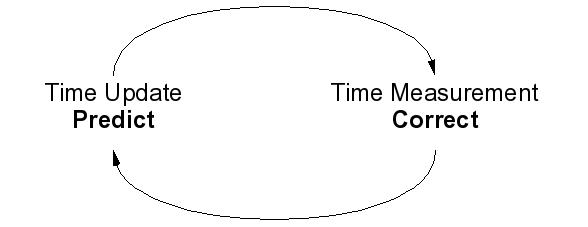
\includegraphics[scale=0.25]{../relazione/figure/PredCorr.jpg}
\caption{\textit{Il ciclio di calcolo del filtro di Kalman.}}
\end{figure}}
%%%%%%%%%%%%%%%%%%%%%%%%%%%%%%%%%%%%%%%%%%
\frame{\frametitle{ConDensation}
\begin{itemize}
 \item Algoritmo probabilistico (aka \textit{Particle Filter})
\item Robusto su rumore e cambiamenti di stato non lineari
\item Campionamento su $N$ samples, applicato alla teoria probabilistica
\end{itemize}
\begin{block}


\begin{itemize}
\item $H_{t}$: samples all'istante $t$.
 \{$\overrightarrow{s_1}(t),\overrightarrow{s_1}(t),...,\overrightarrow{s_N}(t)$\}
\item Samples: $\overrightarrow{s_i}(t)= \{\overrightarrow{x_i}(t),p(x_i(t))$\}
\end{itemize}
% Qui si parla delle funzioni di ogni matrice...
\end{block}
%\begin{figure}[hb]
\centering
	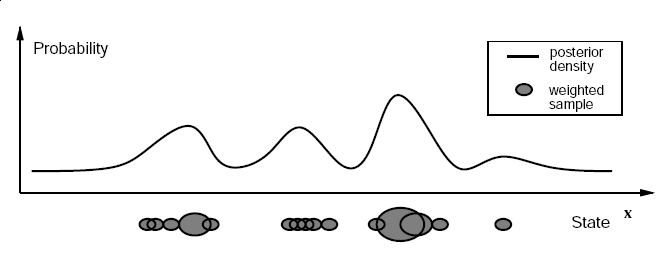
\includegraphics[scale=0.3]{../relazione/figure/samplesProb.png}
%\caption{\textit{Samples e relative probabilità}}
%\end{figure}

\begin{block}{}
Predizione: $\overrightarrow{s_i}(t)$ con probabilità maggiore
\end{block}

}
%%%%%%%%%%%%%%%%%%%%%%%%%%%%%%%%%%%%%%%%%%

\frame{\frametitle{Implementazione del modello}
\begin{itemize}
\item Studio del modello di caduta di un grave
\item Estensione e progettazione del modello per il moto generico di un oggetto su un piano cartesiano
\begin{itemize}
\item $ \Rightarrow$ Scrittura delle matrici del sistema dinamico da usare come input nell'applicativo.
\end{itemize}

\end{itemize}

\begin{block}{Matrici d'interesse del sistema dinamico}
$\overrightarrow{x}=\begin{bmatrix} x \\ y \\ v_x \\ v_y \end{bmatrix}$
$ A = 
\begin{bmatrix}
 1 & 0 & \Delta t & 0 \\
 0 & 1 & 0 & \Delta t \\
 0 & 0 & 1 & 0 \\
 0 & 0 & 0 & 1
\end{bmatrix}$
$Q = 0.01 \cdot Id $
\end{block}




}
%%%%%%%%%%%%%%%%%%%%%%%%%%%%%%%%%%%%%%%%%%
\section{Software}
\frame{\frametitle{Librerie e background subtraction}

\begin{itemize}
\item OpenCV, librerie per \textit{computer vision} di Intel sotto licenza open source.
\item Sotware crossplatform scritto in C++
\end{itemize}

\begin{block}{Background subtraction MoG}
Mixture of Gaussian
\begin{itemize}
\item efficiente anche su video complessi
\item \textit{tuning} dei parametri come:
\begin{itemize}
 \item Soglia di classificazione
\item Numero di Gaussiane per pixel
\end{itemize}


\end{itemize}
\end{block}


}
%%%%%%%%%%%%%%%%%%%%%%%%%%%%%%%%%%%%%%%%%%
\begin{frame}[fragile]
\frametitle{Control-flow}

\textit{Steps} effettuati durante l'esecuzione:

\begin{itemize}
\item Apertura del video da filesystem e ottenimento delle informazioni
\item Ciclo su tutti frame del video:
	\begin{enumerate}
	\item Background Subtraction
	\item Aggiornamento di Kalman e Condensation
	\item Rappresentazione dei risultati 
	\end{enumerate}
\end{itemize}

\begin{figure}[hb]
\centering
	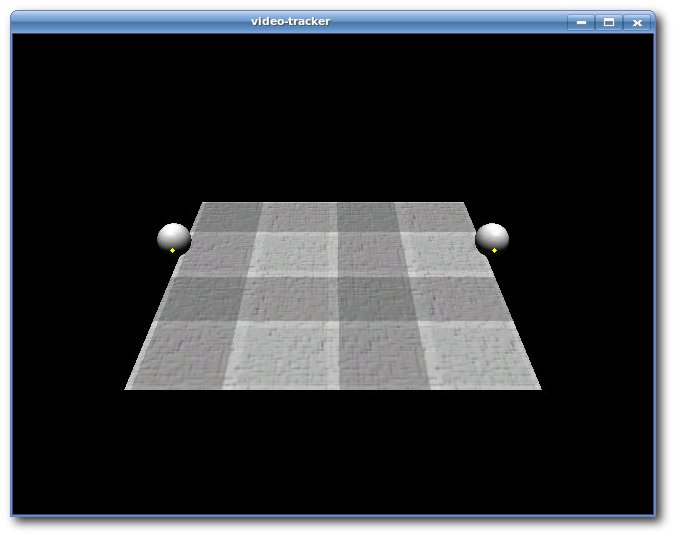
\includegraphics[scale=0.2]{../relazione/figure/doppiascelta.jpg}
\caption[Esempio di scelta tra due blob]{\textit{Detecting di più blob durante tracking multiplo.}\label{fig:scelta2blob}}
\end{figure}

%\lstset{language=c++}
%\lstset{commentstyle=\emph}
%\begin{lstlisting}[frame=tr,breaklines=true,basicstyle=\tiny]
%	video = captureFromAvi( file )
%	initBackgroundSubtraction( video )

%	for( int fr = 1; frame = captureNextFrame( video ), fr++ ){
%	
%                updateBackgroundSubtraction( frame )
%		
%                if ( frame == FIRST_FRAME){
%			
%                        blob = getBlobSelectedFromUser( frame )
%	
%                        initKalman( blob );
%			
 %                       initCondensation( blob );
  %              }
   %             else{
    %            blob= getBlob(Frame);
     %           updateKalman(blob);
      %          updateCondensation(blob);
       %         }
       % }
%\end{lstlisting}



\end{frame}
%%%%%%%%%%%%%%%%%%%%%%%%%%%%%%%%%%%%%%%%%%
\section{Esperimenti}
\frame{\frametitle{Primo video - movie12.mjpeg}
\begin{columns}
\column{.65\textwidth}
\begin{small}\begin{itemize}
 \item occlusione, moto circolare e costante
\item 640x480, 25$fps$, 50.4$s$
\end{itemize}\end{small}

\column{.35\textwidth}\centering
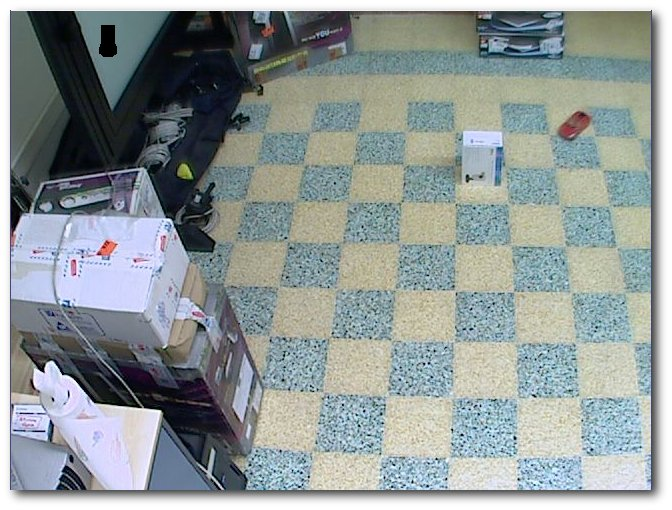
\includegraphics[scale=0.15]{../relazione/figure/movie12.jpg}
\end{columns}
\begin{columns}

\column{.20\textwidth}
\begin{scriptsize}
\begin{itemize}
\item [M]3
\item [Q]1000
\item [S]1000
\end{itemize}
\end{scriptsize}
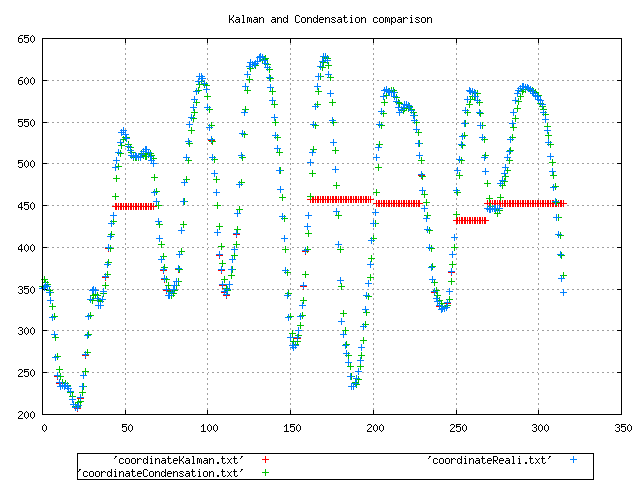
\includegraphics[scale=0.1]{../esperimenti/movie12/mod_3-Q_1000-S_1000/plot.png}\\
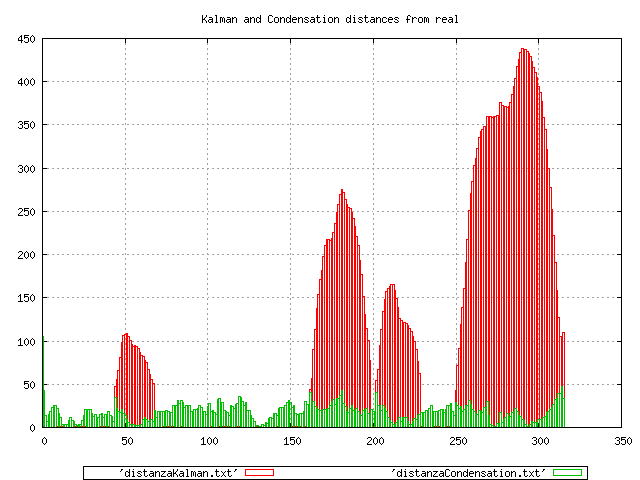
\includegraphics[scale=0.1]{../esperimenti/movie12/mod_3-Q_1000-S_1000/plot-distances.png}

\column{.20\textwidth}
\begin{scriptsize}
\begin{itemize}
\item [M]3
\item [Q]2000
\item [S]1000
\end{itemize}
\end{scriptsize}
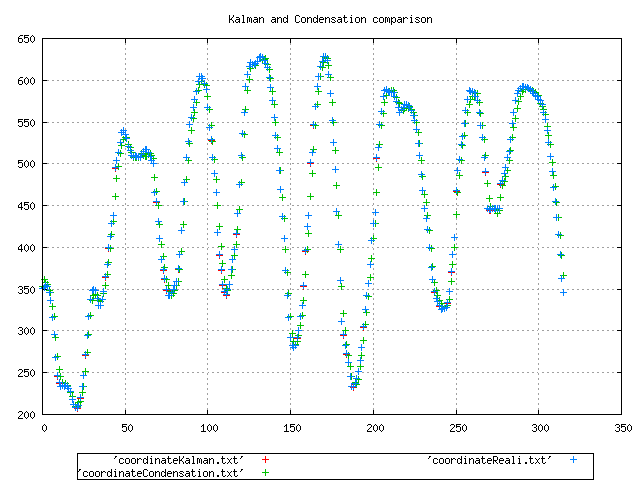
\includegraphics[scale=0.1]{../esperimenti/movie12/mod_3-Q_2000-S_1000/plot.png}\\
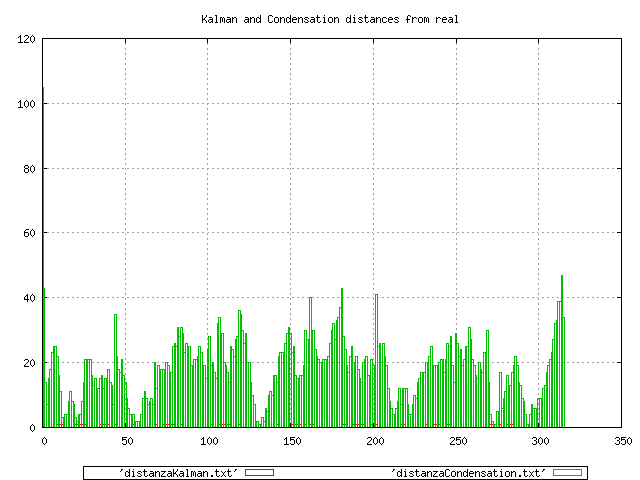
\includegraphics[scale=0.1]{../esperimenti/movie12/mod_3-Q_2000-S_1000/plot-distances.png}

\column{.20\textwidth}
\begin{scriptsize}
\begin{itemize}
\item [M]3
\item [Q]1000
\item [S]5000
\end{itemize}
\end{scriptsize}
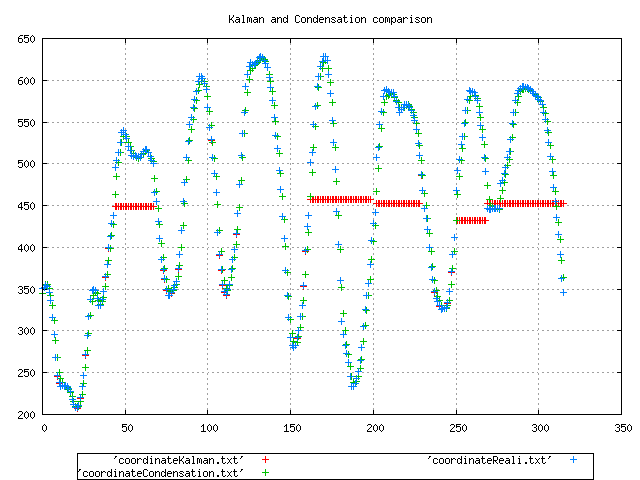
\includegraphics[scale=0.1]{../esperimenti/movie12/mod_3-Q_1000-S_5000/plot.png}\\
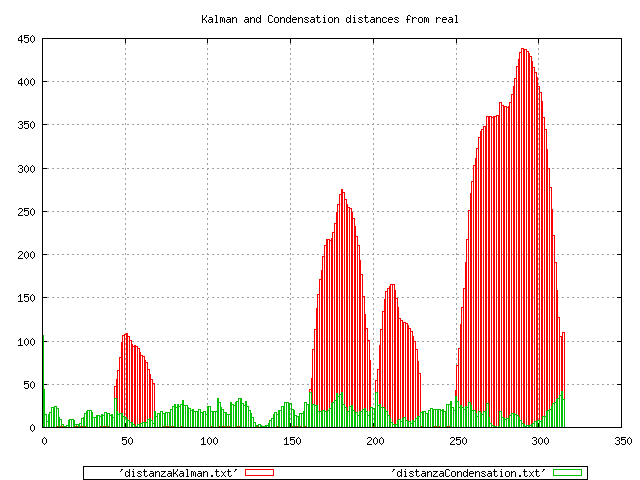
\includegraphics[scale=0.1]{../esperimenti/movie12/mod_3-Q_1000-S_5000/plot-distances.png}

\column{.20\textwidth}
\begin{scriptsize}
\begin{itemize}
\item [M]3
\item [Q]1000
\item [S]100
\end{itemize}
\end{scriptsize}
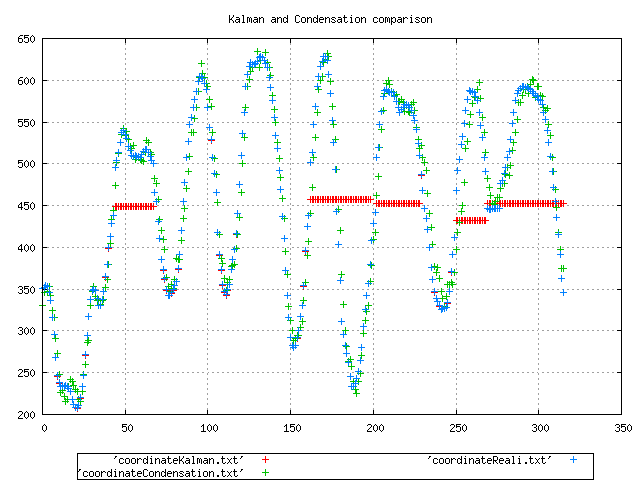
\includegraphics[scale=0.1]{../esperimenti/movie12/mod_3-Q_1000-S_100/plot.png}\\
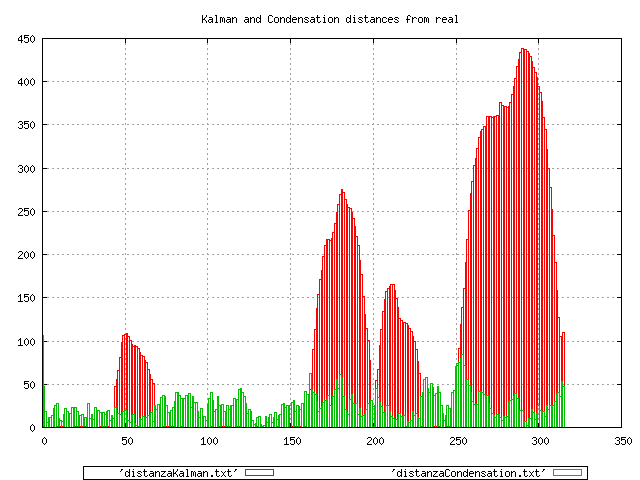
\includegraphics[scale=0.1]{../esperimenti/movie12/mod_3-Q_1000-S_100/plot-distances.png}
\end{columns}

}
%%%%%%%%%%%%%%%%%%%%%%%%%%%%%%%%%%%%%%%%%%
\frame{\frametitle{Secondo video - tappetonomod.avi}
\begin{columns}
\column{.65\textwidth}
\begin{small}\begin{itemize}
 \item moto vario, repentine accelerazioni, oggetto entra ed esce dalla scena
\item 320x240, 10$fps$, 60$s$
\end{itemize}\end{small}

\column{.35\textwidth}\centering
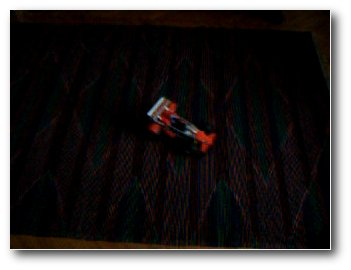
\includegraphics[scale=0.25]{../relazione/figure/tappeto_nomod.jpg}
\end{columns}
\begin{columns}

\column{.20\textwidth}
\begin{scriptsize}
\begin{itemize}
\item [M]3
\item [Q]1000
\item [S]1000
\end{itemize}
\end{scriptsize}
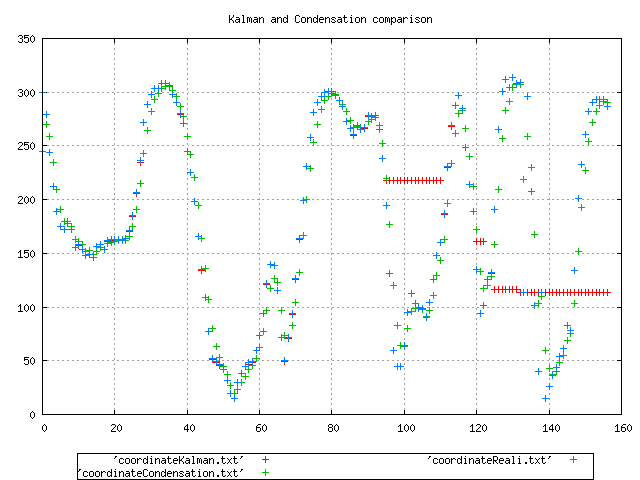
\includegraphics[scale=0.1]{../esperimenti/tappeto_nozoom/mod_3-Q_1000-S_1000/plot.png}\\
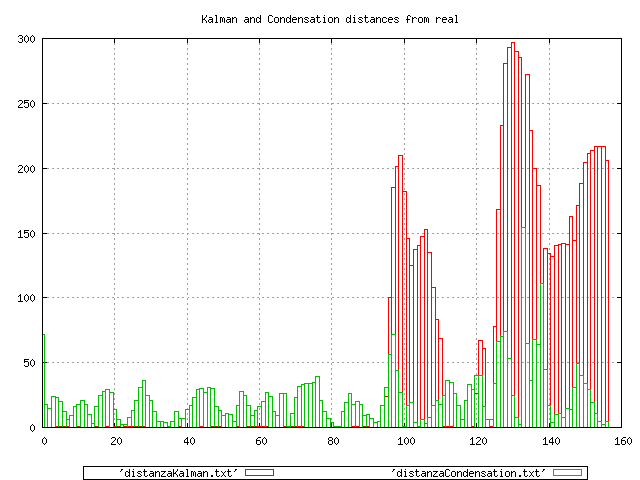
\includegraphics[scale=0.1]{../esperimenti/tappeto_nozoom/mod_3-Q_1000-S_1000/plot-distances.png}

\column{.20\textwidth}
\begin{scriptsize}
\begin{itemize}
\item [M]5
\item [Q]1000
\item [S]1000
\end{itemize}
\end{scriptsize}
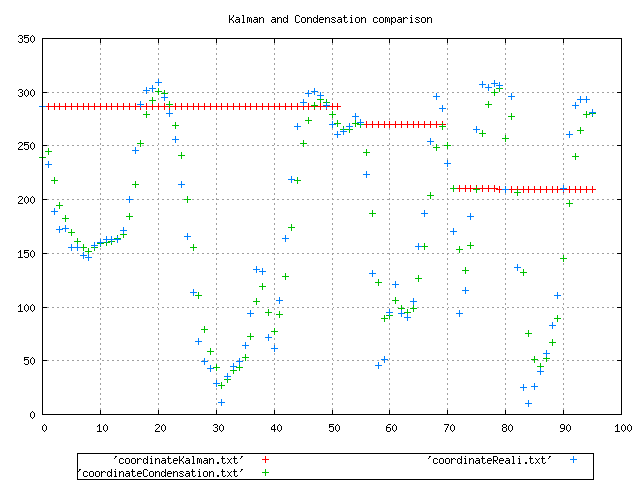
\includegraphics[scale=0.1]{../esperimenti/tappeto_nozoom/mod_5-Q_1000-S_1000/plot.png}\\
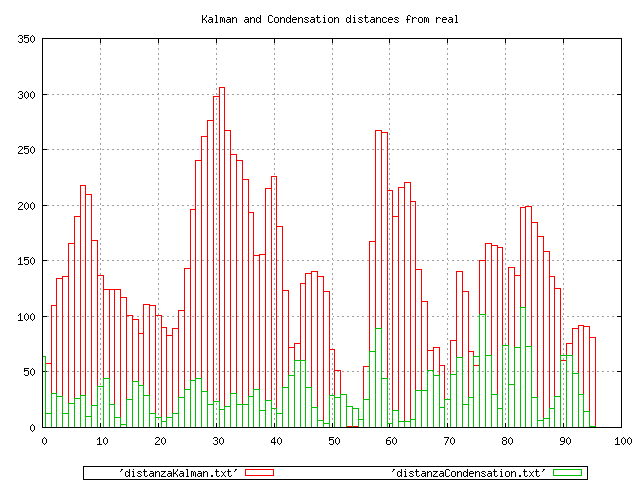
\includegraphics[scale=0.1]{../esperimenti/tappeto_nozoom/mod_5-Q_1000-S_1000/plot-distances.png}


\column{.20\textwidth}
\begin{scriptsize}
\begin{itemize}
\item [M]2
\item [Q]1000
\item [S]1000
\end{itemize}
\end{scriptsize}
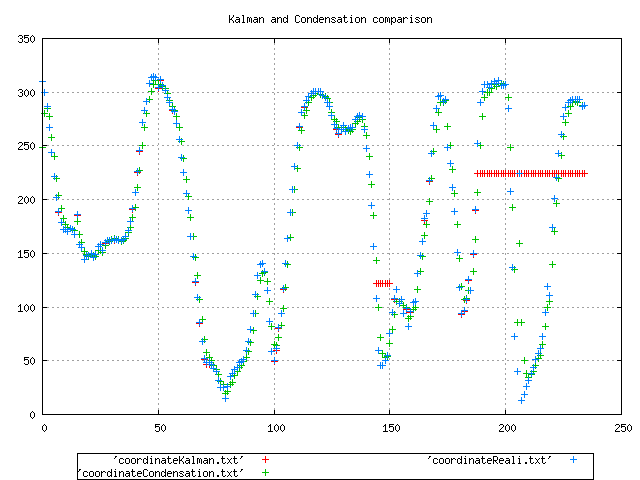
\includegraphics[scale=0.1]{../esperimenti/tappeto_nozoom/mod_2-Q_1000-S_1000/plot.png}\\
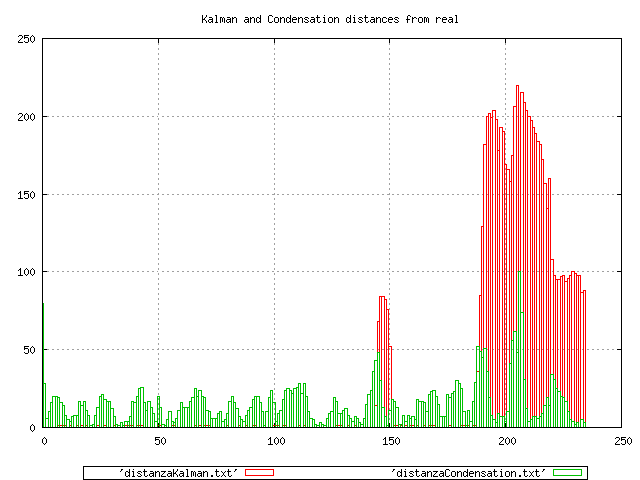
\includegraphics[scale=0.1]{../esperimenti/tappeto_nozoom/mod_2-Q_1000-S_1000/plot-distances.png}


\column{.20\textwidth}
\begin{scriptsize}
\begin{itemize}
\item [M]1
\item [Q]2000
\item [S]1000
\end{itemize}
\end{scriptsize}
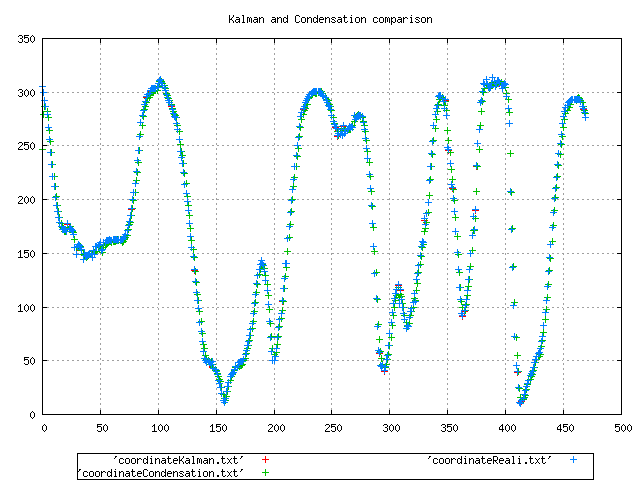
\includegraphics[scale=0.1]{../esperimenti/tappeto_nozoom/mod_1-Q_2000-S_1000/plot.png}\\
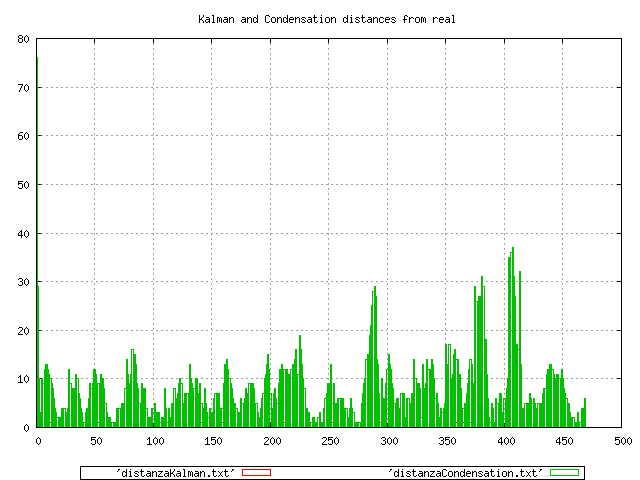
\includegraphics[scale=0.1]{../esperimenti/tappeto_nozoom/mod_1-Q_2000-S_1000/plot-distances.png}
\end{columns}

}
%%%%%%%%%%%%%%%%%%%%%%%%%%%%%%%%%%%%%%%%%%
\frame{\frametitle{Terzo video - singlecar.avi}
\begin{columns}
\column{.65\textwidth}
\begin{small}\begin{itemize}
 \item moto costante, oggetto entra ed esce dalla scena
\item 648x484, 30$fps$, 33$s$
\end{itemize}\end{small}

\column{.35\textwidth}\centering
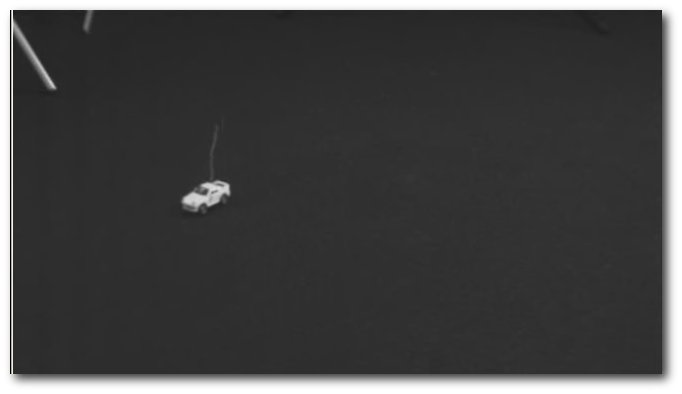
\includegraphics[scale=0.15]{../relazione/figure/singlecar.jpg}
\end{columns}
\begin{columns}

\column{.20\textwidth}
\begin{scriptsize}
\begin{itemize}
\item [M]3
\item [Q]1000
\item [S]1000
\end{itemize}
\end{scriptsize}
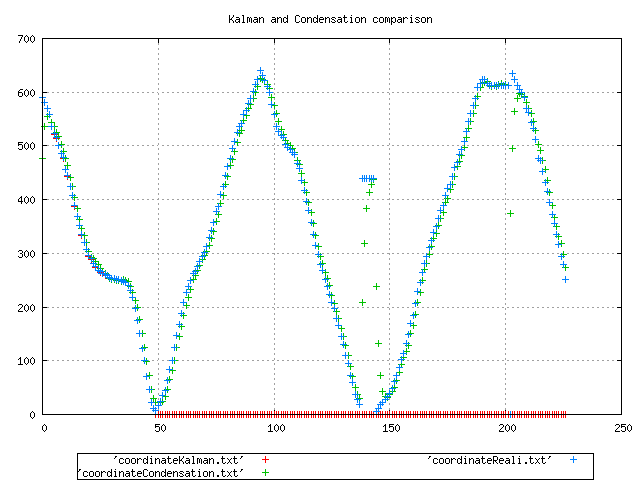
\includegraphics[scale=0.1]{../esperimenti/single_car/mod_3-Q_1000-S_1000/plot.png}\\
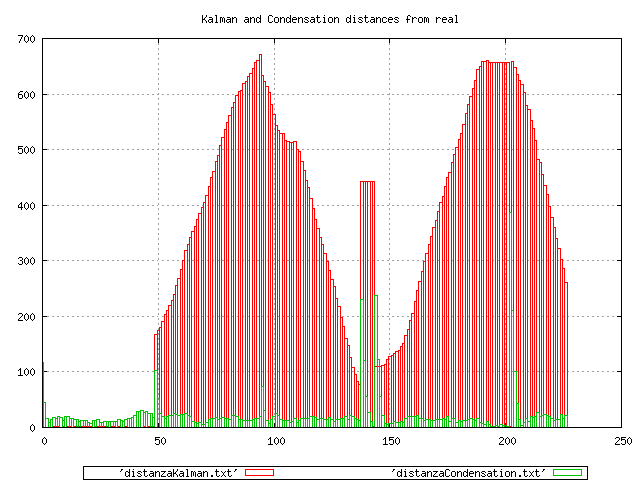
\includegraphics[scale=0.1]{../esperimenti/single_car/mod_3-Q_1000-S_1000/plot-distances.png}

\column{.20\textwidth}
\begin{scriptsize}
\begin{itemize}
\item [M]10
\item [Q]5000
\item [S]1000
\end{itemize}
\end{scriptsize}
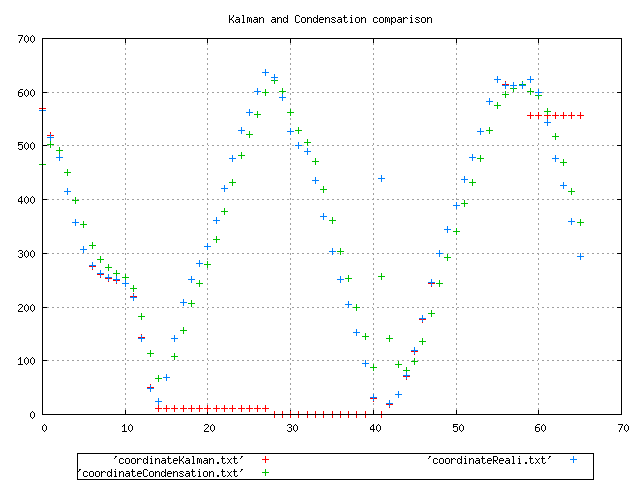
\includegraphics[scale=0.1]{../esperimenti/single_car/mod_10-Q_5000-S_1000/plot.png}\\
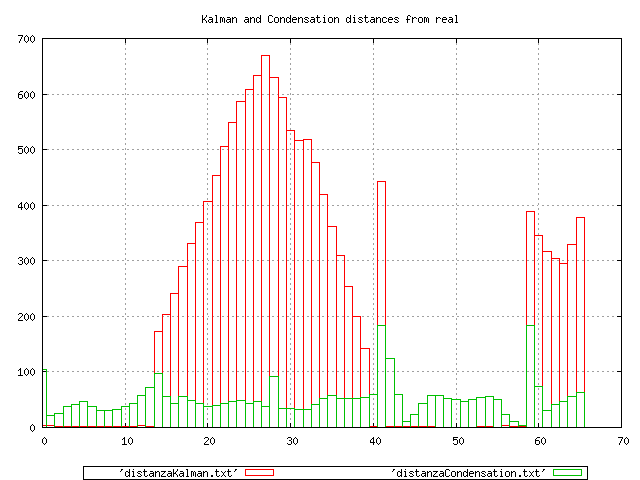
\includegraphics[scale=0.1]{../esperimenti/single_car/mod_10-Q_5000-S_1000/plot-distances.png}

\column{.20\textwidth}
\begin{scriptsize}
\begin{itemize}
\item [M]6
\item [Q]0.1
\item [S]1000
\end{itemize}
\end{scriptsize}
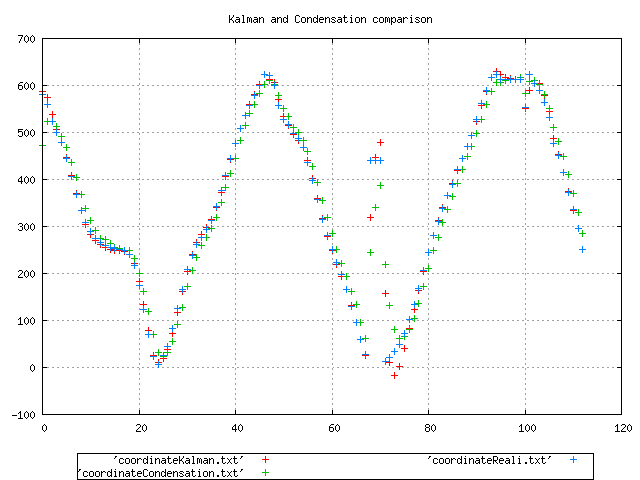
\includegraphics[scale=0.1]{../esperimenti/single_car/mod_6-Q_0.1-S_1000/plot.png}\\
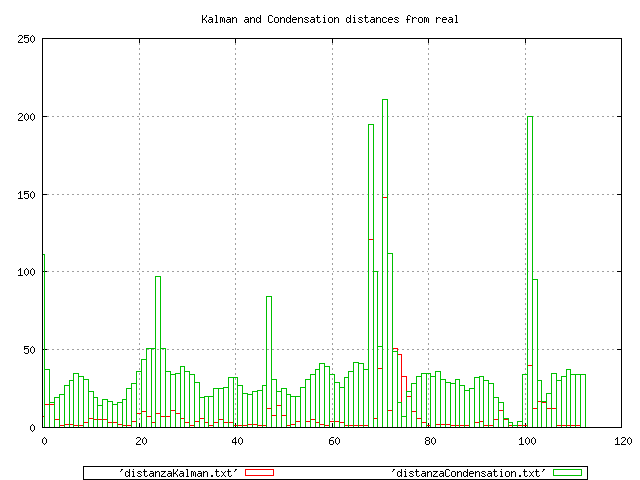
\includegraphics[scale=0.1]{../esperimenti/single_car/mod_6-Q_0.1-S_1000/plot-distances.png}

\column{.20\textwidth}
\begin{scriptsize}
\begin{itemize}
\item [M]1
\item [Q]0.0001
\item [S]1000
\end{itemize}
\end{scriptsize}
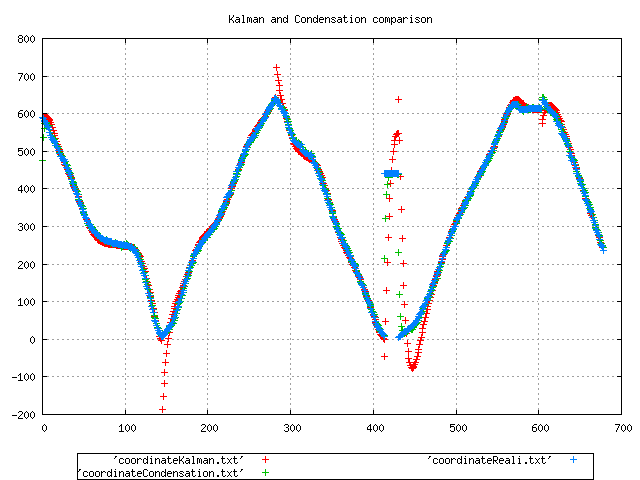
\includegraphics[scale=0.1]{../esperimenti/single_car/mod_1-Q_0.0001-S_1000/plot.png}\\
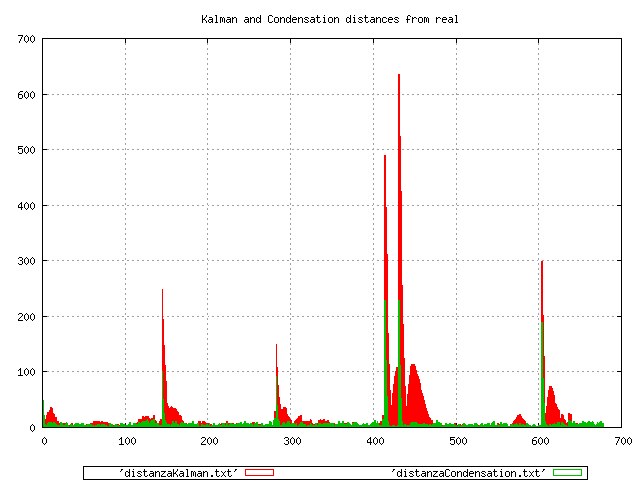
\includegraphics[scale=0.1]{../esperimenti/single_car/mod_1-Q_0.0001-S_1000/plot-distances.png}
\end{columns}
}
%%%%%%%%%%%%%%%%%%%%%%%%%%%%%%%%%%%%%%%%%%
\section{Conclusione}
%%%%%%%%%%%%%%%%%%%%%%%%%%%%%%%%%%%%%%%%%
\frame{\setbeamercolor{titlelike}{bg=UNL@Scarlet,fg=UNL@Cream}
\vspace{-10pt}
\begin{center}
\begin{scriptsize}
	\textsc{Università degli studi di Firenze}
\end{scriptsize}\\ 
\begin{tiny}
	Facoltà di Ingegneria - Corso di laurea specialistica in \textsc{Ingegneria Informatica}
\vspace{-20pt}
\end{tiny}
\end{center}

\titlepage
 }
\end{document}
